\documentclass[aspectratio=169]{beamer}

\usepackage{fontspec}
\usepackage{polyglossia}
\usepackage{color}
\usepackage{listings}
\setdefaultlanguage{russian}
\usepackage{csquotes}
\usetheme{metropolis}
\metroset{background=light}
\metroset{sectionpage=none}
\metroset{numbering=fraction}

\definecolor{ssaublue}{RGB}{77,144,205}
\setbeamercolor{frametitle}{fg=white, bg=ssaublue}
\setbeamercolor{title separator}{fg=ssaublue}

\setmainfont[
    Path = ../fonts/elektratextpro/,
    Extension = .otf,
    UprightFont = elektratextpro,
    BoldFont = elektratextpro_bold,
    ItalicFont = elektratextpro_italic,
    BoldItalicFont = elektratextpro_bolditalic
]{elektratextpro}

\setsansfont[
    Path = ../fonts/elektratextpro/,
    Extension = .otf,
    UprightFont = elektratextpro,
    BoldFont = elektratextpro_bold,
    ItalicFont = elektratextpro_italic,
    BoldItalicFont = elektratextpro_bolditalic
]{elektratextpro}

\setmonofont[
    Path = ../fonts/elektratextpro/,
    Extension = .otf,
    UprightFont = elektratextpro,
    BoldFont = elektratextpro_bold,
    ItalicFont = elektratextpro_italic,
    BoldItalicFont = elektratextpro_bolditalic
]{elektratextpro}

\newfontfamily\cyrillicfont[
    Path = ../fonts/elektratextpro/,
    Extension = .otf,
    UprightFont = elektratextpro,
    BoldFont = elektratextpro_bold,
    ItalicFont = elektratextpro_italic,
    BoldItalicFont = elektratextpro_bolditalic
]{elektratextpro}

\newfontfamily\cyrillicfontsf[
    Path = ../fonts/elektratextpro/,
    Extension = .otf,
    UprightFont = elektratextpro,
    BoldFont = elektratextpro_bold,
    ItalicFont = elektratextpro_italic,
    BoldItalicFont = elektratextpro_bolditalic
]{elektratextpro}

\newfontfamily\cyrillicfonttt[
    Path = ../fonts/elektratextpro/,
    Extension = .otf,
    UprightFont = elektratextpro,
    BoldFont = elektratextpro_bold,
    ItalicFont = elektratextpro_italic,
    BoldItalicFont = elektratextpro_bolditalic
]{elektratextpro}

% Настройка листингов для Beamer
\lstset{
    basicstyle=\ttfamily\footnotesize,
    commentstyle=\color{gray},
    columns=fullflexible,
    keepspaces=true,
    breaklines=false,
    extendedchars=true,
    texcl=true,
    showstringspaces=false
}

\title{Cloud computing}
\date{12 ноября 2025 г.}

\begin{document}
    \maketitle

    \begin{frame}{Модели размещения ИТ инфраструктуры}
        \begin{center}
            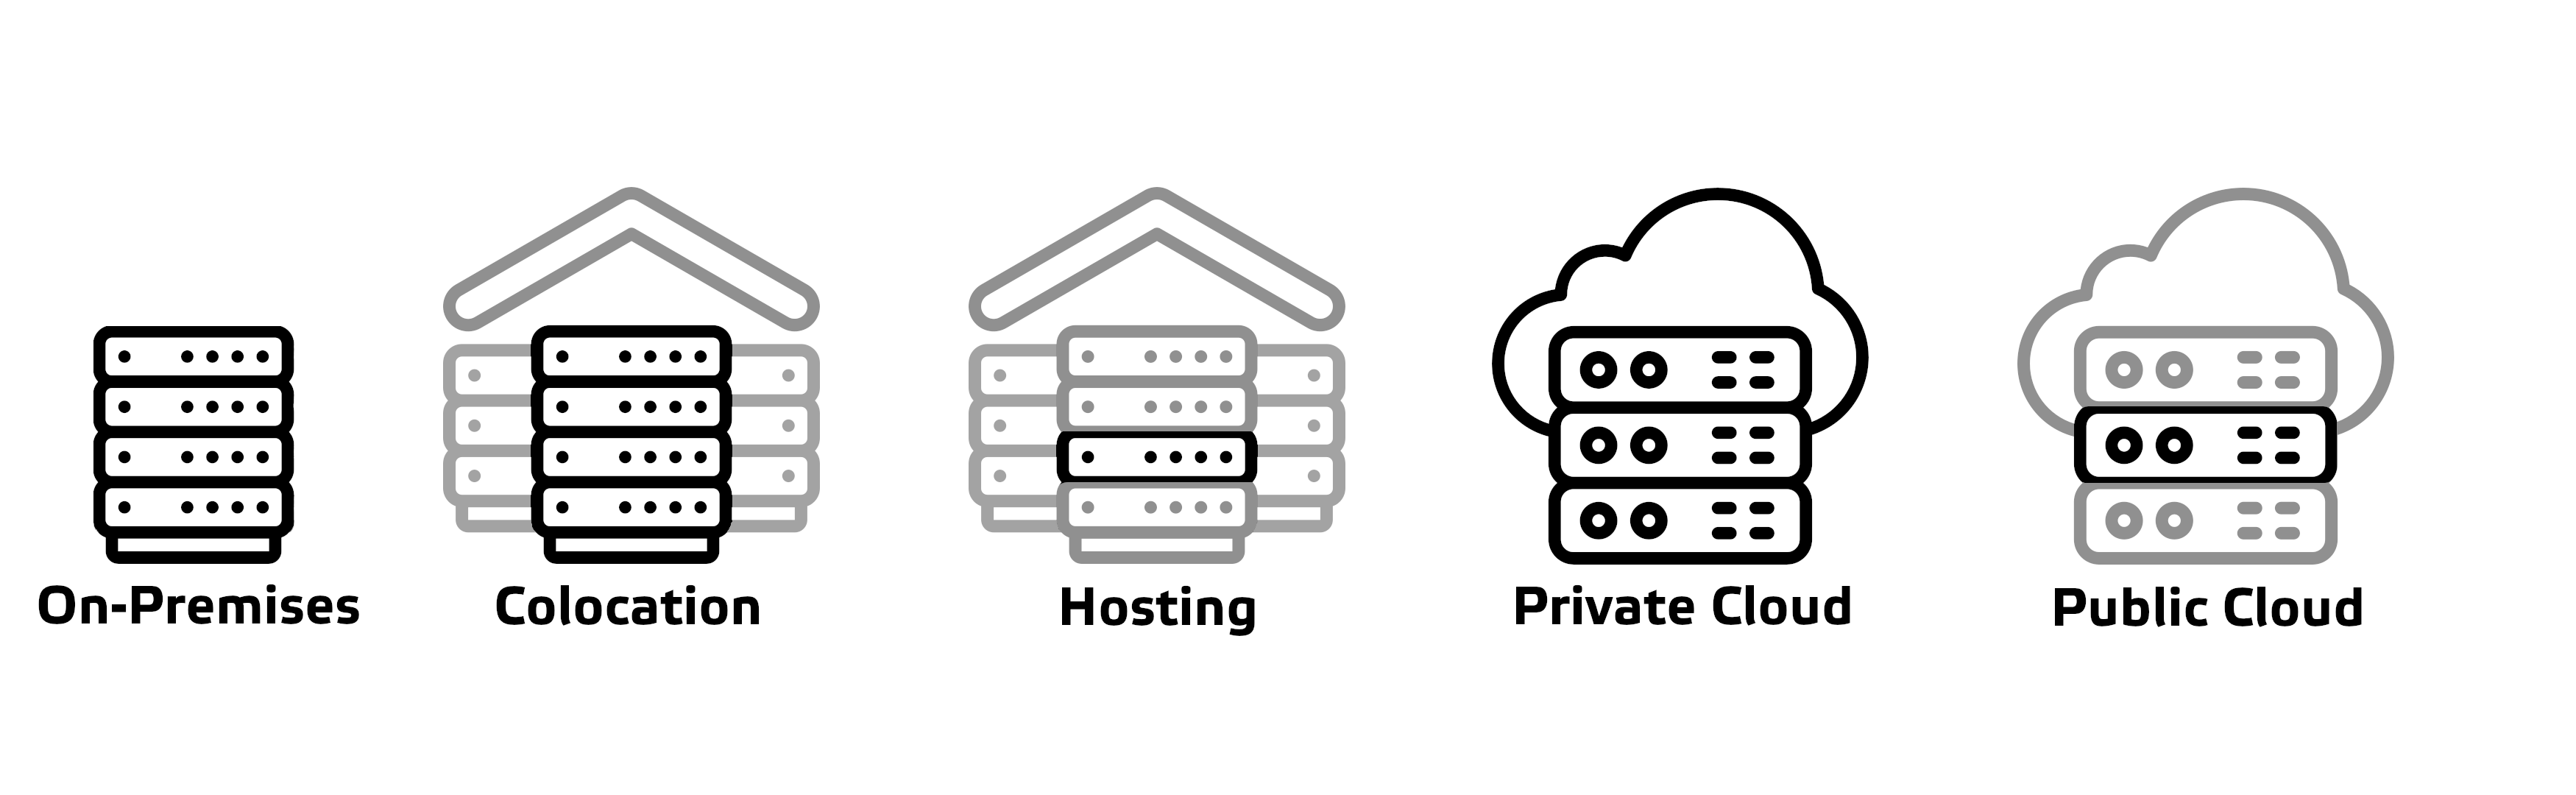
\includegraphics[width=1\textwidth]{media/infras}
        \end{center}
    \end{frame}

    \begin{frame}{Cloud}
        Cloud - это модель предоставления и использования вычислительных ресурсов по запросу.

        \vspace{0.3cm}

        Public Cloud провайдер - внешняя компания

        Private Cloud провайдер - внутренняя ИТ-служба

        \vspace{0.3cm}

        Преимущества:
        \begin{enumerate}
            \item Гибкость и масштабируемость
            \item Экономичность
            \item Быстрое развертывание
            \item Надёжность и отказоустойчивость
            \item Безопасность
        \end{enumerate}
    \end{frame}

    \begin{frame}{Private vs Public}
        \begin{columns}[t]
            \begin{column}[t]{0.465\textwidth}
                \textbf{Private Cloud:}
                \begin{itemize}
                    \item VMware vSphere
                    \item OpenStack
                    \item Proxmox
                \end{itemize}
            \end{column}

            \begin{column}[t]{0.465\textwidth}
                \textbf{Public Cloud:}
                \begin{itemize}
                    \item AWS
                    \item Azure
                    \item Google Cloud
                    \item Yandex Cloud
                    \item Cloud.ru
                    \item VK Cloud
                \end{itemize}
            \end{column}
        \end{columns}
    \end{frame}

    \begin{frame}{Основные модели облачных услуг}
        \begin{center}
            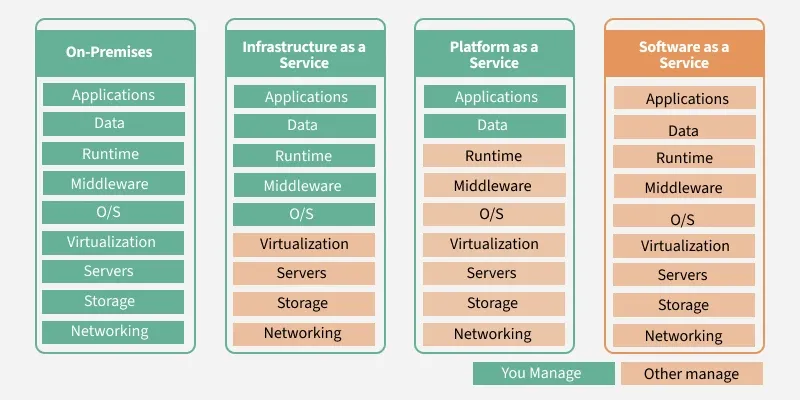
\includegraphics[width=0.85\textwidth]{media/iaas_paas_saas}
        \end{center}

        \footnotesize{\textcolor{gray}{\href{https://www.geeksforgeeks.org/software-engineering/difference-between-iaas-paas-and-saas/}{https://www.geeksforgeeks.org/software-engineering/...}}}
    \end{frame}

    \begin{frame}{*aaS}
        \begin{itemize}
            \item FaaS
            \item KaaS
            \item CaaS
            \item DBaaS
        \end{itemize}
    \end{frame}

    \begin{frame}{Yandex Cloud}
        \href{https://yandex.cloud/ru/docs/overview/concepts/services}{Список сервисов}
        \href{https://yandex.cloud/ru/docs/getting-started/usage-grant}{Стартовый грант}
    \end{frame}

    \begin{frame}{Демонстрация: сервисы в Yandex Cloud}
        \begin{itemize}
            \item \href{https://yandex.cloud/ru/docs/compute/}{Yandex Compute Cloud}
            \item \href{https://yandex.cloud/ru/docs/storage/}{Yandex Object Storage}
            \item \href{https://yandex.cloud/ru/docs/functions/}{Yandex Cloud Functions}
            \item \href{https://yandex.cloud/ru/docs/ydb/}{Yandex Managed Service for YDB}
            \item \href{https://yandex.cloud/ru/docs/cloud-apps/}{Cloud Apps}
        \end{itemize}
    \end{frame}

    \begin{frame}{Ссылки по теме}
        \begin{itemize}
            \item \url{https://www.theguardian.com/technology/2009/sep/02/cory-doctorow-cloud-computing}
            \item \url{https://zegetech.com/blog/2018/11/12/cloud-cloud-computing.html}
        \end{itemize}
    \end{frame}
\end{document}